%TEX root = ../dissertation.tex

\chapter{Background and Literature Review}
\label{chapter:Background}
    
This chapter provides a theoretical basis to help understand the Machine Learning Model used as well as the matter under study in this thesis. The first two subsections, \ref{sec:machine_learning} and \ref{sec:neural_networks}, outline the general topic of Machine Learning and the specific area of Deep Learning models. These subsections cover feature engineering, training of machine learning algorithms, the concept of loss, the feed-forward network and multilayered neural networks. The third subsection, \ref{AE_VAE}, explains the theoretical foundation of autoencoders and more specifically variational autoencoders, the architecture of the model which this thesis is based on. Section \ref{chapter:Uncertainty} serves to explain the general concept of uncertainty in machine learning as well as the two most commonly identified sources of uncertainty: aleatoric uncertainty and epistemic uncertainty. Section \ref{chapter:MOSA_outline} makes a detailed description of the Multi-Omic Synthetic Augmentation (\gls{MOSA}) model which is the key model studied in this thesis.

\section{Deep Learning Models}

\subsection{Machine Learning} \label{sec:machine_learning}

Machine Learning is a subfield of artificial intelligence that is concerned with the training of algorithms and statistical models that automatically learn from data to carry out a given task.  In contemporary data-driven applications, Machine Learning can be interpreted as finding functional relationships between input  and output variables when explicit analytical modelling is too complex or uncertain.

The central challenge in Machine Learning is being able to represent data in a way that allows for an algorithm to learn from it. Raw data rarely possesses the required structure for effective model training and generalisation. This brings about the need for feature engineering, the process of transforming the original raw data into informative, compact and discriminative features that potentiate learning the given task. From a theoretical perspective, learning algorithms operate in a hypothesis space $\mathcal{H}$ defined over feature vectors $\mathbf{x} \in \mathbb{R}^d$. The choice of feature mapping $\phi: \mathcal{X} \rightarrow \mathbb{R}^d$ directly influences the complexity of the hypothesis space \cite{Hastie2009}. Inadequate feature selection can make the target function unrepresentable within $\mathcal{H}$, regardless of the learning algorithm employed, while choosing excessively complex features may lead to overfitting and poor model generalisation. Feature engineering and selection can thus be interpreted as an implicit form of inductive bias, which encodes domain knowledge into the learning process, aiming to reduce sample complexity and improve robustness \cite{Bishop2006}. 

Learning in Machine Learning is typically formulated as an optimisation problem. Given a data set $\{(\mathbf{x}_i, y_i)\}_{i=1}^n$ drawn from an unknown joint distribution $p(\mathbf{x}, y)$, the objective is to find a function $f_\theta \in \mathcal{H}$ parameterised by $\theta$ that minimises the expected risk

\[
\mathcal{R}(\theta) = \mathbb{E}_{(\mathbf{x}, y) \sim p} \left[ \ell(f_\theta(\mathbf{x}), y) \right],
\]

where $\ell(\cdot,\cdot)$ is a loss function that quantifies the discrepancy between predictions and true outcomes \cite{Vapnik1998}. Since the true distribution is unknown, the expected risk is approximated by the empirical risk
\begin{equation}
\hat{\mathcal{R}}(\theta) = \frac{1}{n} \sum_{i=1}^n \ell(f_\theta(\mathbf{x}_i), y_i).
\end{equation}
The choice of loss function is problem-dependent and encodes assumptions about noise, error tolerance, and the statistical properties of the data. For example, the squared loss $\ell(y,\hat{y}) = (y-\hat{y})^2$ corresponds to maximum likelihood estimation under Gaussian noise assumptions, while the cross-entropy loss arises from a Bernoulli or categorical likelihood in classification settings \cite{Bishop2006}.

Machine Learning methods are commonly categorised into three types of learning based on the nature of supervision available during training: supervised, unsupervised and reinforcement learning. In supervised learning, each input is paired with a corresponding target output, enabling direct estimation of input-output mappings. This describes tasks such as classification and regression. In unsupervised learning, the data consist solely of inputs without labelled outputs, and the objective is to uncover latent structures, such as clusters or low-dimensional representations, by modelling the marginal distribution $p(\mathbf{x})$ \cite{Hastie2009}. In reinforcement learning, an agent interacts with an environment by taking actions and receiving scalar rewards, with the goal of learning a policy that maximises expected cumulative reward over time. This setting is formalised using Markov decision processes and differs fundamentally from supervised learning due to delayed feedback and the exploration-exploitation dilemma \cite{Sutton2018}. Despite their differences, all three paradigms can be unified under the perspective of optimisation and statistical inference.

Within supervised learning, classification and regression represent two fundamental problem classes distinguished by the nature of the target variable. In regression, the target $y \in \mathbb{R}$ is continuous, and the goal is to approximate a real-valued function. In classification, the target variable takes values in a finite set of discrete classes.  From a statistical decision theory perspective, both regression and classification aim to approximate the Bayes optimal predictor that minimises expected loss, differing primarily in the loss function and output space.

\begin{figure}
    \centering
    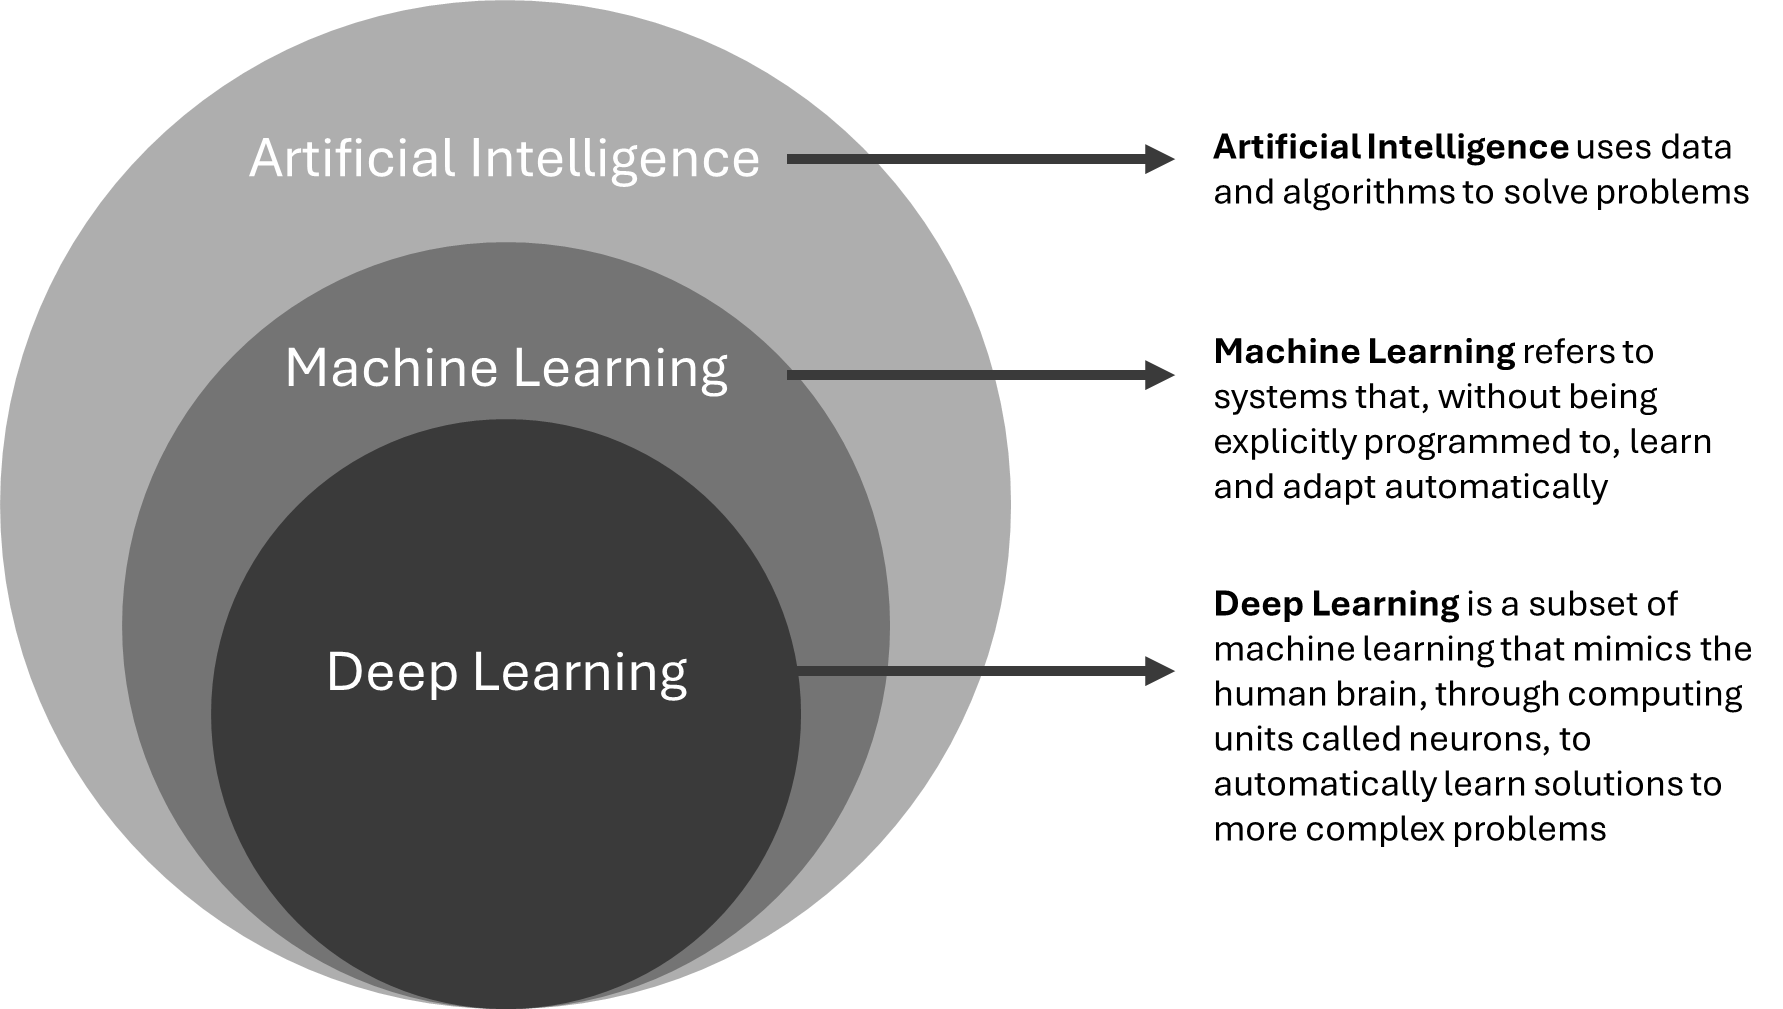
\includegraphics[width=0.75\linewidth]{images/AI_ML_DL_2.png}
    \caption[AI, machine learning and deep learning relationship illustration]{Illustration of relationship between Artificial Intelligence, Machine Learning and Deep Learning}
    \label{fig:AI_ML_DL}
\end{figure}

\subsection{Neural Networks} \label{sec:neural_networks}

Neural networks constitute a central class of models within modern Machine Learning and form the conceptual and practical foundation of deep learning. Artificial neural networks are composed of connected layered nodes that transform input data through successive non-linear operations. The defining characteristic of deep learning lies in the use of multiple layers of representation, enabling the hierarchical extraction of features and the approximation of highly complex functions \cite{Goodfellow2016}. From a theoretical standpoint, deep neural networks can be understood as function approximators whose ability to express information extracted from data grows with depth, allowing them to model compositional structures that are difficult or inefficient to capture with simpler architectures \cite{Telgarsky2016}.

The fundamental building block of neural networks is the perceptron, originally introduced as a simplified model of a biological neuron \cite{Rosenblatt1958}. The perceptron computes a weighted sum of its input features $\mathbf{x} \in \mathbb{R}^d$, adds a bias term $b \in \mathbb{R}$, and applies an activation function $g(\cdot)$, yielding an output
\begin{equation}
y = g(\mathbf{w}^\top \mathbf{x} + b),
\end{equation}
where $\mathbf{w} \in \mathbb{R}^d$ denotes the weight vector.  While this model is capable of learning linearly separable functions, it is fundamentally limited in representational capacity, as famously demonstrated by its inability to represent non-linearly separable functions such as the exclusive-or (XOR) problem \cite{Minsky1969}. This limitation highlighted the necessity of extending the perceptron model beyond a single unit.

The introduction of multiple layers of perceptrons leads to the \gls{MLP}, which overcomes the representational constraints of single-layer models. An MLP consists of an input layer, one or more hidden layers, and an output layer, where each layer applies an affine transformation followed by a non-linear activation function. Formally, for a network with $L$ layers, the forward computation can be expressed recursively as
\begin{equation}
\mathbf{h}^{(l)} = g^{(l)}\left( \mathbf{W}^{(l)} \mathbf{h}^{(l-1)} + \mathbf{b}^{(l)} \right), \quad l = 1, \dots, L,
\end{equation}

with $\mathbf{h}^{(0)} = \mathbf{x}$. The composition of non-linear transformations enables the network to approximate a wide class of functions. The universal approximation theorem states that a feedforward neural network with at least one hidden layer and a sufficient number of units can, in principle, approximate any continuous function to any desired degree of accuracy \cite{Cybenko1989}. Depth, however, offers practical advantages by achieving similar expressivity with fewer parameters and improved generalisation in many settings \cite{Goodfellow2016}. An example of a simple feedforward network can be seen in Figure \ref{fig:mlp}.

\begin{figure}
    \centering
    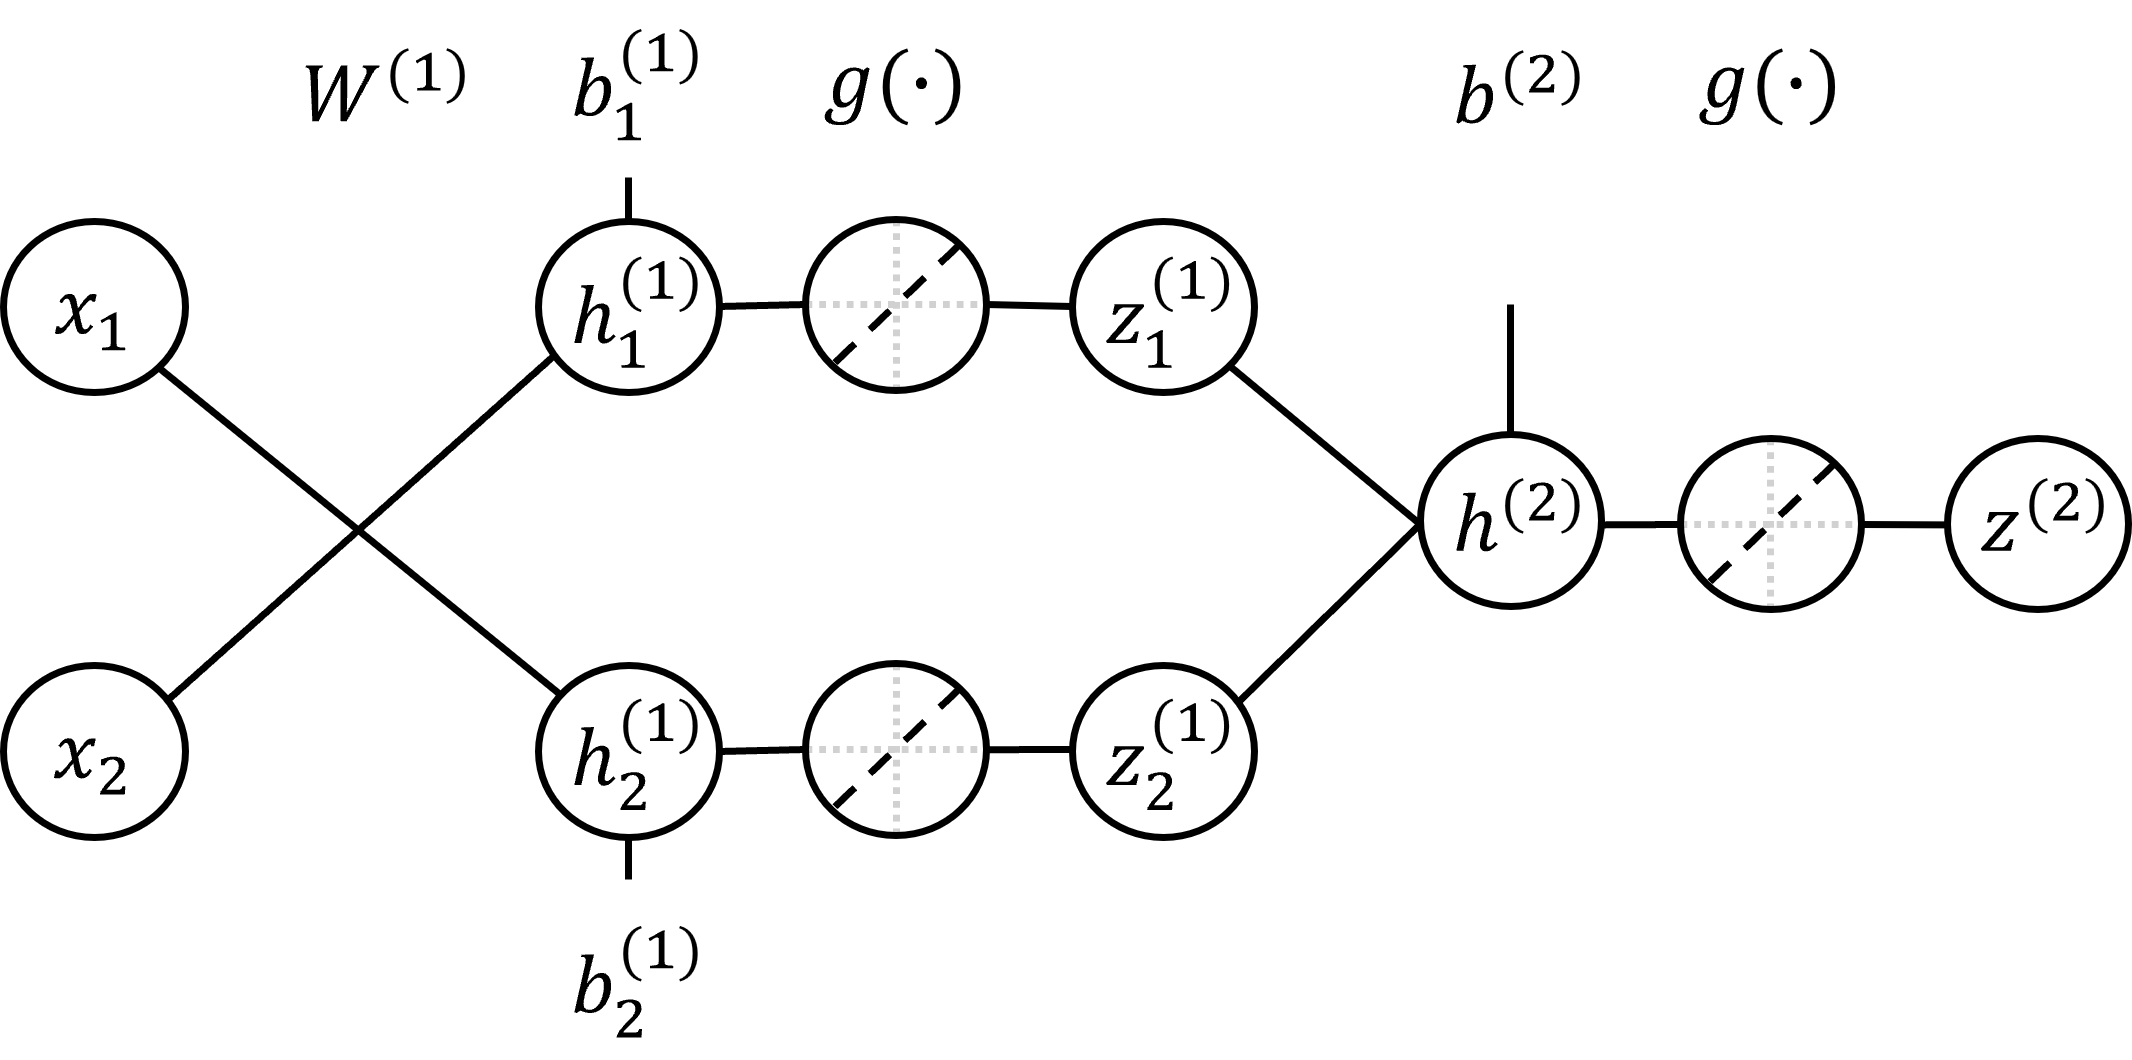
\includegraphics[width=0.75\linewidth]{images/Perceptron.png}
    \caption{Feed-Forward Network with one hidden layer and two neurons.}
    \label{fig:mlp}
\end{figure}

The computation performed by an MLP during inference is referred to as the feedforward mechanism. In this phase, information flows from the input layer to the output layer, with each layer transforming the representation produced by the previous one. The feedforward pass defines the mapping from inputs to predictions and is purely deterministic given the network parameters. Training the network requires adjusting these parameters to minimise a predefined loss function, which is accomplished through backpropagation combined with gradient-based optimisation. Backpropagation is an application of the chain rule of calculus that computes gradients of the loss function with respect to each parameter in the network \cite{Rumelhart1986}. Given a loss $\ell(\hat{y}, y)$, the gradient with respect to parameters in layer $l$ depends on gradients from subsequent layers, allowing error signals to be propagated backward through the network.

Once gradients are computed, parameters are updated using gradient descent or one of its variants. In its basic form, gradient descent updates parameters according to

\begin{equation}
    \theta_{t+1} = \theta_t - \eta \nabla_\theta \hat{\mathcal{R}}(\theta_t),
\end{equation}

where $\theta$ denotes the collection of all weights and biases, $\eta$ is the learning rate, and $\hat{\mathcal{R}}$ is the empirical risk \cite{Bishop2006}. In practice, stochastic gradient descent and its adaptive extensions are commonly employed to scale training to large datasets and deep architectures. The interaction between backpropagation and gradient descent constitutes the core learning mechanism of neural networks and enables optimisation of complex, multilayer models.

Despite their expressive power, neural networks are prone to overfitting, particularly when trained on limited data with a large number of parameters. Regularisation techniques are therefore essential to improve generalisation. Classical approaches include $\ell_2$ regularisation, which penalises large weights by adding a term $\lambda \|\theta\|_2^2$ to the loss function, effectively constraining the capacity of the model \cite{Hastie2009}. Another widely used technique is dropout, which randomly deactivates a subset of neurons during each training iteration \cite{Srivastava2014}. Dropout can be interpreted as implicitly training an ensemble of subnetworks and has been shown to reduce co-adaptation of features, thereby enhancing robustness. Additional regularisation strategies, such as early stopping and normalisation techniques, further contribute to stabilising training and improving performance.

\subsection{Autoencoders and Variational Autoencoders} \label{AE_VAE}


Autoencoders constitute an important deep learning architecture design for learning. These models learn data representations in an unsupervised manner by constraining the information flow through the network using a lower-dimensional bottleneck. Formally, given input data \(x \in \mathbb{R}^d\), an autoencoder comprises an encoder function \(f_\phi : \mathbb{R}^d \rightarrow \mathbb{R}^k\) and a decoder function \(g_\theta : \mathbb{R}^k \rightarrow \mathbb{R}^d\), parameterised by \(\phi\) and \(\theta\) respectively, where \(k < d\) defines the latent representation dimensionality. The encoder maps the input data to a latent code \(h = f_\phi(x)\), and the decoder attempts to reconstruct the original input as \(\hat{x} = g_\theta(h)\) \cite{Goodfellow2016}. Training occurs by minimising a reconstruction loss over a dataset \(\{x_i\}_{i=1}^N\), such as the mean squared error,
\begin{equation}
    \mathcal{L}_{\text{AE}}(\theta,\phi) = \frac{1}{N}\sum_{i=1}^N \lVert x_i - g_\theta(f_\phi(x_i)) \rVert_2^2,
\end{equation}
or a suitable alternative, chosen based on the data type and output distribution. The bottleneck allows the network to compress the input \(x\) into a compact representation, which preserves the information most relevant for reconstructing the data. The resulting latent codes can be interpreted as non-linear features adapted to the structure of the dataset \cite{Goodfellow2016}. An illustration of a standard Autoencoder can be seen in Figure \ref{fig:autoencoder}.

\begin{figure}[!ht]
    \centering
    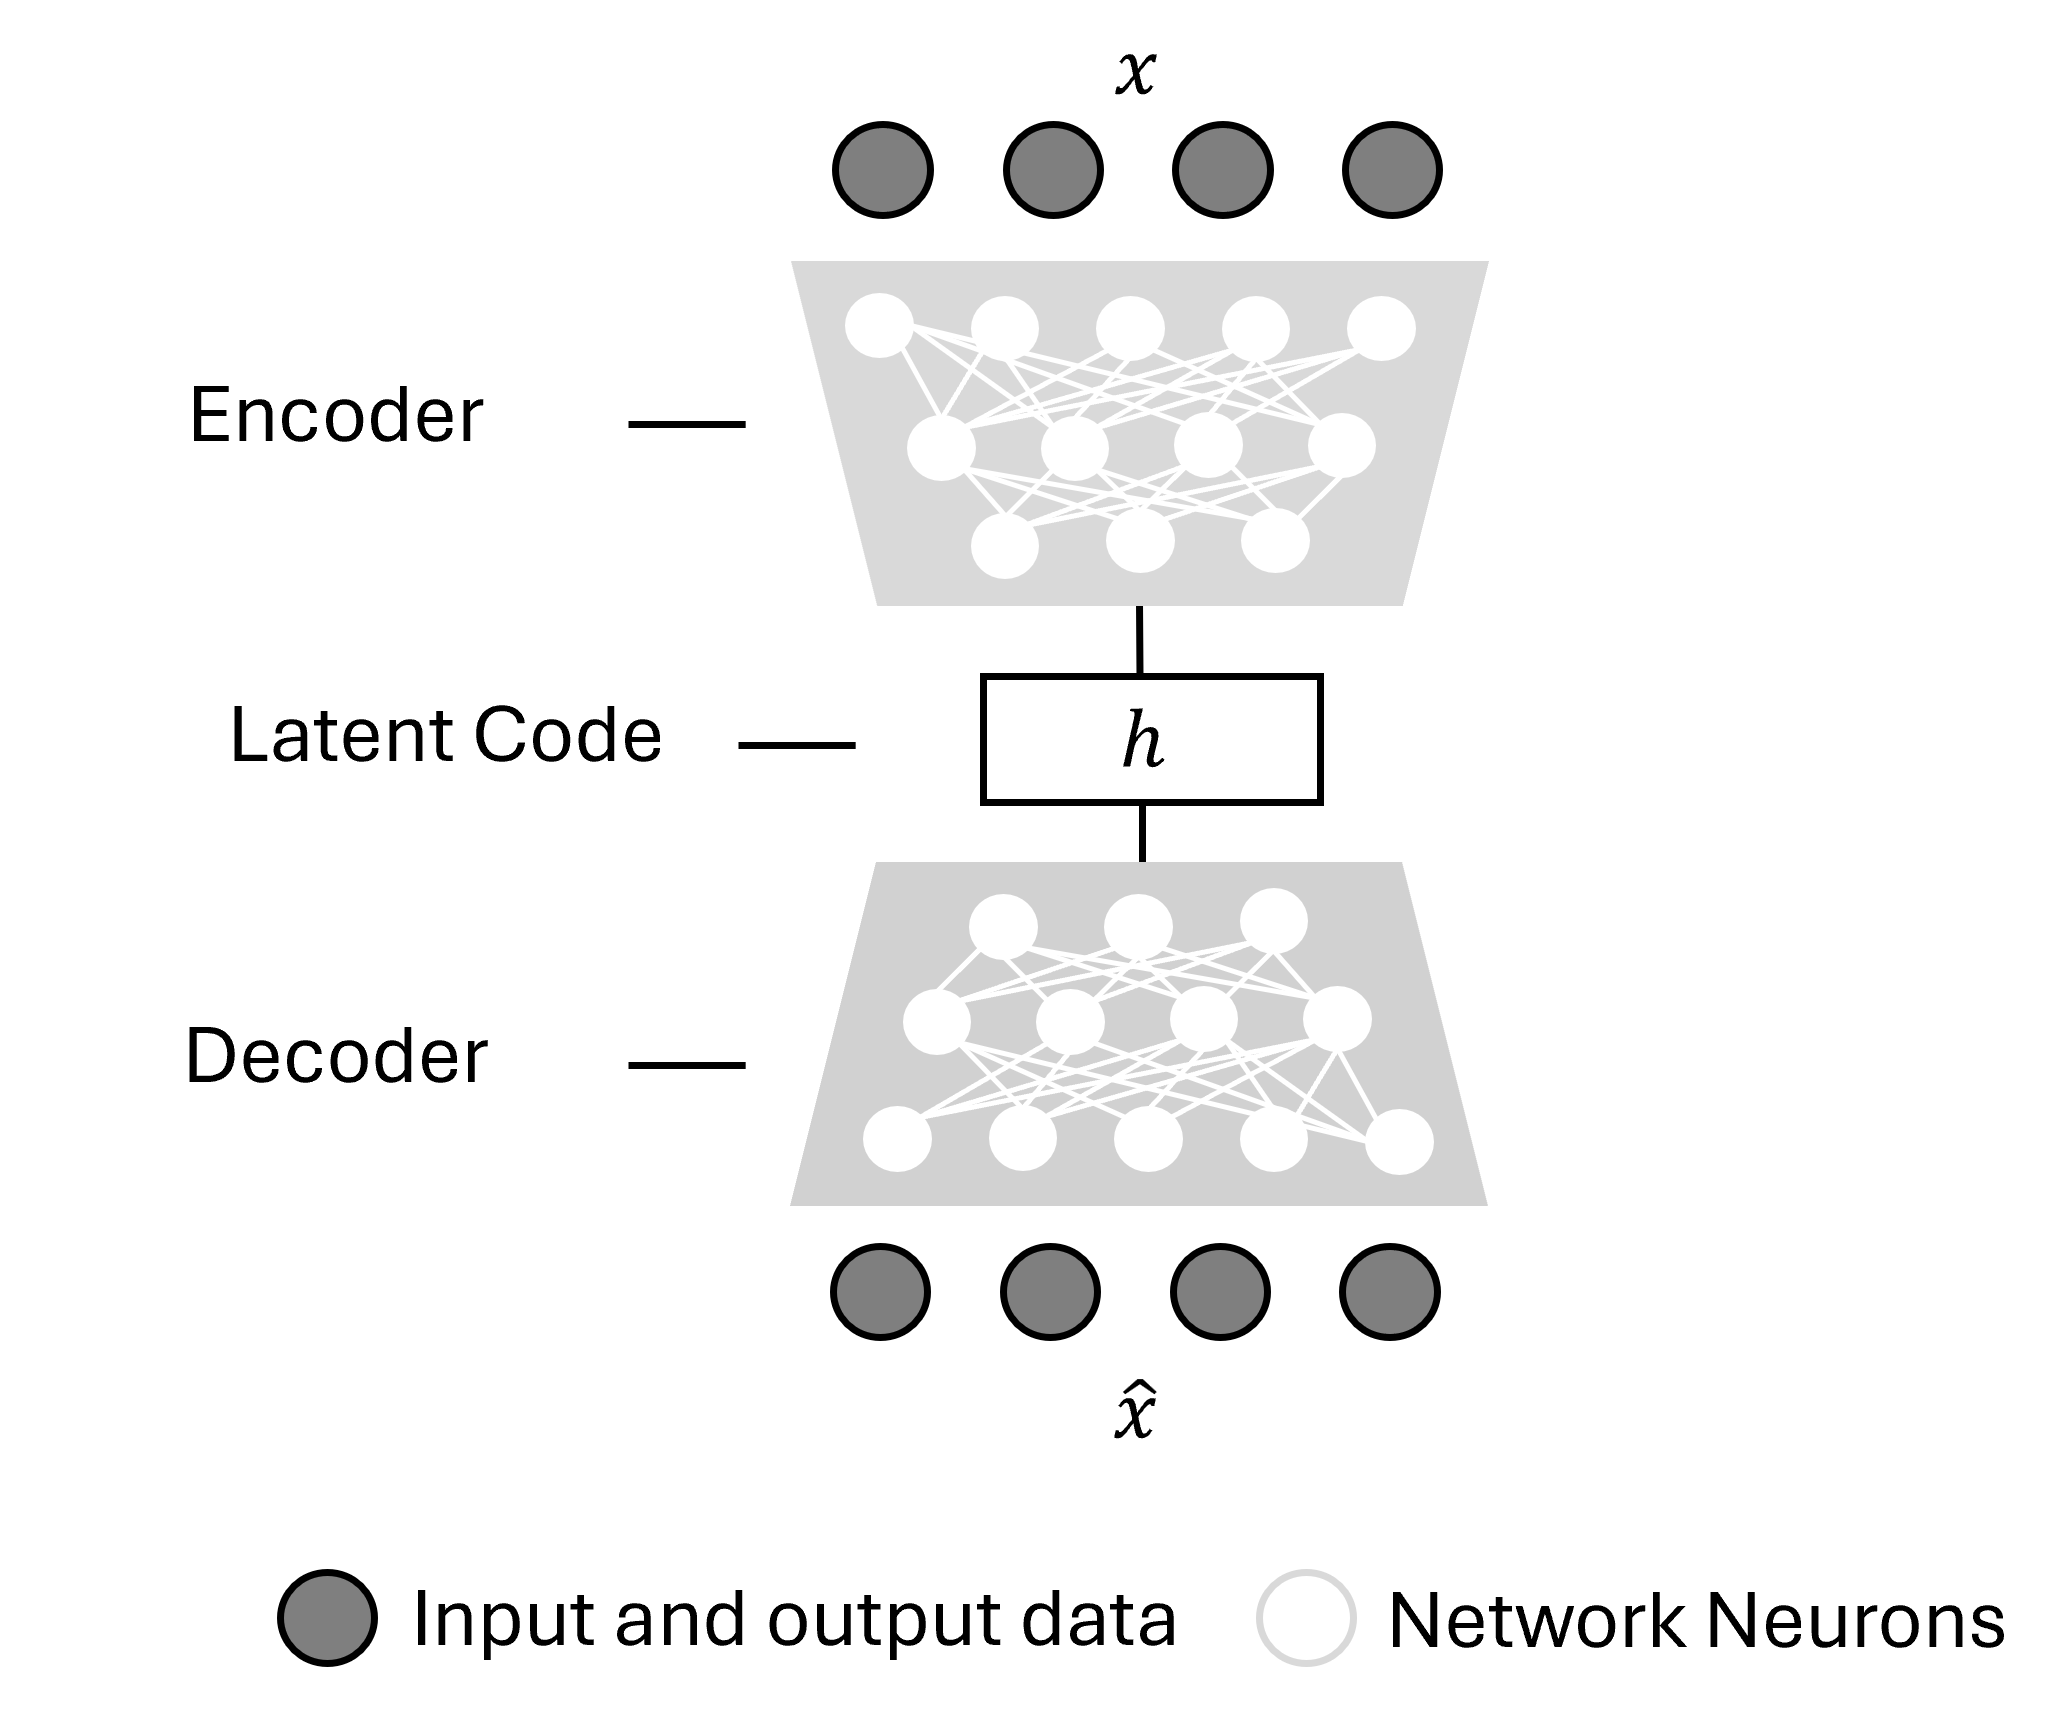
\includegraphics[width=0.5\linewidth]{images/AutoEncoder.png}
    \caption{Illustration of the standard Autoencoder architecture.}
    \label{fig:autoencoder}
\end{figure}

Beyond the basic undercomplete architecture, additional regularisation mechanisms have been introduced to provide autoencoders with desirable properties such as robustness to noise or sparsity in the representation. While the variants obtained by adding these mechanisms enhance the quality of learned representations, classical autoencoders remain primarily deterministic reconstruction models. This means that they do not define an explicit generative model over observations, limiting the ability of the model to generate novel data \cite{Goodfellow2016}.

\Glspl{VAE} address this limitation by turning the autoencoder architecture into a probabilistic latent-variable model. Instead of an encoder's deterministic latent code, a VAE learns a distribution over latent variables using this distribution to reconstruct observations or generate new data. This model architecture assumes a joint distribution \(p_\theta(x,z)=p_\theta(x\mid z)p(z)\), where \(z\) is a latent variable, \(p(z)\) is typically a standard normal prior \(\mathcal{N}(0,I)\), and \(p_\theta(x\mid z)\) is a likelihood defined by the decoder \cite{Kingma2013AutoEncodingVB}. This way the VAE can learn parameters \(\theta\) such that the marginal likelihood
\begin{equation}
    p_\theta(x) = \int p_\theta(x \mid z)p(z)\,dz
\end{equation}
approximates the original data's distribution. Usually, directly optimising this likelihood is intractable as the true posterior \(p_\theta(z\mid x)\) cannot be computed analytically. VAEs address this issue using variational inference.

An encoder defines an approximate posterior \(q_\phi(z\mid x)\), which is trained to approximate the intractable true posterior. Training maximises the \gls{ELBO},
\begin{equation}
    \mathcal{L}(\theta,\phi; x) = \mathbb{E}_{q_\phi(z \mid x)} \left[ \log p_\theta(x \mid z) \right] - \mathrm{KL}\!\left(q_\phi(z \mid x) \,\|\, p(z)\right),
\end{equation}
which satisfies \(\log p_\theta(x) \geq \mathcal{L}(\theta,\phi;x)\) \cite{Kingma2013AutoEncodingVB}. The first term is a reconstruction term, which encourages the decoder to assign high likelihood to the input when decoding latent samples from \(q_\phi(z\mid x)\). The second term is the Kullback-Leibler (KL) divergence between the approximate posterior and the prior. It regularises the latent space by discouraging \(q_\phi(z\mid x)\) from getting too far from \(p(z)\). This makes it possible to sample \(z\sim p(z)\) and decode it into plausible novel data. This means that the ELBO balances reconstruction quality against latent-space regularity.

The reparameterisation trick makes this objective practical to optimise with gradient descent. Instead of directly sampling \(z\) from \(q_\phi(z\mid x)\), the encoder outputs distribution parameters. Commonly these parameters are a distribution's mean \(\mu_\phi(x)\) and standard deviation \(\sigma_\phi(x)\). A sample is then written as
\begin{equation}
    z = \mu_\phi(x) + \sigma_\phi(x) \odot \epsilon,
\end{equation}
where \(\epsilon \sim \mathcal{N}(0,I)\) \cite{Kingma2013AutoEncodingVB}. This expresses the random sample as a differentiable transformation of the encoder outputs and an external noise variable, allowing gradients to flow through the sampling step during backpropagation.

This probabilistic structure gives VAEs a smoother and more organised latent space than standard autoencoders. Interpolations between latent codes can produce meaningful changes in the decoded output, and variants such as \(\beta\)-VAE modify the KL term to encourage more disentangled latent representations. Despite this, VAEs also have limitations. Expressive decoders may lead to posterior collapse, where the latent variables are largely ignored. These issues have motivated more expressive likelihoods, hierarchical latent variables, modified objectives, and hybrid models such as VAE-GANs \cite{Kingma2013AutoEncodingVB,Higgins2017betaVAE}.

\section{Uncertainty in Machine Learning}  \label{chapter:Uncertainty}

In machine learning, predictive uncertainty refers to the ambiguity of the posterior predictive distribution for a given input. It arises from insufficient training data, noisy or incomplete observations, poor model quality and from a mismatch between the training distribution and real data. A deterministic neural network trained through risk minimisation typically produces point estimates of its parameters and point predictions at test time. Such outputs, however, do not by themselves quantify the degree to which a prediction is affected by noise in the observations, lack of data, or poor learned parameters. For this reason, uncertainty in deep learning is naturally formulated in terms of the predictive distribution rather than a single predicted value \cite{kendall2017uncertainties,mena2021survey}.

Let \(x\) denote an input, \(y\) a target variable, \(\theta\) the model parameters, and \(\mathcal{D}\) the training dataset. In a probabilistic setting, prediction is described by the posterior predictive distribution

\begin{equation}
p(y \mid x, \mathcal{D}) = \int p(y \mid x, \theta)\, p(\theta \mid \mathcal{D})\, d\theta .
\end{equation}

This expression shows that predictive uncertainty arises from at least two conceptually distinct sources. The term \(p(y \mid x, \theta)\) represents uncertainty inherent in the conditional relation between input and output data, whereas the posterior \(p(\theta \mid \mathcal{D})\) represents uncertainty induced by incomplete knowledge of the model after training on finite data \cite{kendall2017uncertainties}. In the literature, these two sources are conventionally referred to as aleatoric uncertainty and epistemic uncertainty \cite{derkiureghian2009aleatory,kendall2017uncertainties}.

Aleatoric uncertainty is associated with irreducible variability inherent to the data gathering process or to the data itself. In the classical uncertainty literature, it corresponds to randomness intrinsic to a phenomenon \cite{derkiureghian2009aleatory}. In deep learning, aleatoric uncertainty arises when the target is noisy, partially observed, ambiguously labelled or corrupted by measurement error \cite{kendall2017uncertainties}. Even if the parameters of the predictor were known, this variability would remain present in the predictive distribution. Aleatoric uncertainty is thus often regarded as irreducible through the collection of additional samples from the same data-generating process \cite{kendall2017uncertainties}. Additional data may improve estimation of this variability, but it does not eliminate the variability itself.

A distinction of practical importance is that between homoscedastic and heteroscedastic forms of aleatoric uncertainty. Homoscedastic uncertainty is constant across the input space and can be represented by a single global noise parameter. Heteroscedastic uncertainty varies with the input and is, therefore, more relevant in modern deep learning applications since the difficulty of prediction is rarely uniform across all regions of the data manifold \cite{kendall2017uncertainties}.

Epistemic uncertainty, on the other hand, is associated with incomplete knowledge of the predictor. It reflects uncertainty about the model parameters, representations or about the effective hypothesis selected during model training \cite{derkiureghian2009aleatory,kendall2017uncertainties}. Unlike with aleatoric uncertainty, epistemic uncertainty is in principle reducible since it decreases as the model is informed by more representative observations, stronger structural assumptions or a better configuration of the model's weights. In deep learning, epistemic uncertainty is especially significant in regions of the input space that are not well supported by the training data. In such regions the learned model needs to extrapolate beyond the empirical evidence that defined its parameters during training. For this reason, epistemic uncertainty is closely related to data scarcity, covariate shift, out-of-distribution inputs, and model misspecification \cite{mena2021survey,jang2023survey}.

The Bayesian framework provides the most direct formalisation of epistemic uncertainty, since the posterior distribution \(p(\theta \mid \mathcal{D})\) quantifies the residual uncertainty over model parameters after data has been observed \cite{jang2023survey}. Exact Bayesian inference is, however, computationally intractable for most neural networks of practical interest. The literature has thus focused on approximate procedures such as variational Bayesian neural networks, Monte Carlo Dropout, Laplace approximations and deep ensembles. These procedures are further discussed in Section \ref{chapter:Literature_Review}.

The distinction between aleatoric and epistemic uncertainty has direct methodological implications because the appropriate response depends on the dominant source of uncertainty. When uncertainty is primarily aleatoric the prediction's limiting factor is the stochastic or ambiguous character of the data collection process. Performance improvements thus require more informative inputs, improved data collection or downstream decisions that explicitly take into account this ambiguity \cite{derkiureghian2009aleatory,kendall2017uncertainties}. When uncertainty is primarily epistemic the more effective solutions are increased coverage of the input space, addition of more representative data in poorly sampled regions or an improvement of the model architecture and parameters \cite{mena2021survey,jang2023survey}.

Calibration methods improve the reliability of these predicted probabilities but do not provide a decomposition of predictive uncertainty into its constituent sources \cite{mena2021survey}. This distinction is important because a model may be well calibrated on in-sample test data while, at the same time, failing to express meaningful epistemic uncertainty on an out-of-sample distributional shift. 

%Com dois subsections mais vale ter só a section em q falo dos dois tipos de incerteza

%Mencionar Out-of-Distribution uncertainty

%\subsection{Aleatoric Uncertainty}

%\subsection{Epistemic Uncertainty}
\section{Methods for Uncertainty Estimation} \label{chapter:Literature_Review}

This section highlights the current state of the art for methods used to ascertain uncertainty in neural networks, the key problem identified in Chapter \ref{chapter:introduction}. %dizer algo mais I guess, tipo 'while there are more methods designed to tackle this problem, they either required a large change in the model arquitecture, defeating the goal of this dissertation, or they ...'
\subsection{Deep Generative Models}

Deep Generative Models (DGMs) are a family of probabilistic models that aim to learn the underlying patterns of data in order to generate new synthetic observations through deep neural network architectures. These models are able to learn tractable latent variables \(z\) from an intractable data distribution with a high-dimensional feature space. This ability to capture probability distributions allows for these models to be used as a way of quantifying uncertainty in a dataset and, additionally, they allow for quantification of uncertainty in these models with little to no adjustments of the model's architecture. State of the art models for uncertainty quantification include Variational Autoencoders, Generative Adversarial Networks (GANs) and diffusion models, but this thesis focuses on VAEs.

Variational autoencoders occupy a central position among uncertainty-aware deep generative models because they make uncertainty explicit through latent-variable probabilistic modelling. As seen in Section \ref{AE_VAE}, VAE specifies a generative model $p_\theta(x,z)=p_\theta(x\mid z)p(z)$ together with an inference model $q_\phi(z\mid x)$, and learning proceeds by maximising a variational lower bound on the log marginal likelihood. Within the contemporary literature, two methods capture much of the state of the art for uncertainty estimation with VAE-based components: probabilistic embeddings for quantifying input uncertainty and conditional VAE formulations for quantifying target prediction uncertainty under ambiguous supervision \cite{Chang2020,Sohn2015}. Hybrid architectures such as the Probabilistic U-Net extend these ideas by combining conditional latent-variable modelling with multi-scale feature extraction for structured outputs \cite{Kohl2018}.

The first method, quantifying input uncertainty through probabilistic embeddings, is motivated by the observation that datasets often contain noise and heterogeneity at the input level. By leveraging the standard VAE architecture we note that the, typically Gaussian, variational latent space contains an embedding distribution where each input sample is mapped to a latent distribution. In the case of a Gaussian latent space, the latent space \(z\) is obtained by sampling from \(\mathcal{N}(\mu(x),\sigma^2(x))\), where \(\mu(x)\) serves as the feature representation and \(\sigma^2(x)\) encodes the uncertainty of the representation. By sampling from the learned latent posterior and decoding these samples we may generate multiple reconstructions of the input data \cite{Edupuganti2021}. This way we take the uncertainty output of the encoder and uncertainty is propagated through the decoder, obtaining both a measure of input uncertainty and model reconstruction uncertainty. This method's limitations are thus that embedding variance may partially contain model uncertainty, dataset bias or training objective artifacts rather than purely reflecting input noise. Similarly, the uncertainty that may be calculated from decoding latent space samples is a composite of both data and model uncertainty.

The second method, quantifying prediction uncertainty, addresses ambiguity in the data reconstruction rather than noise only in the input. In a regular VAE, the latent variable $z$ is used to model variability in the data's distribution $p_\theta(x)$, and the encoder learns $q_\phi(z\mid x)$ so that $z$ captures global components of variability for the input alone. At test time one typically samples $z\sim q_\phi(z\mid x)$ or from the prior $p(z)$ and decodes to reconstruct the input data. By contrast, a cVAE explicitly models the conditional distribution over outputs given inputs. Additionally, the latent space is now designed to capture residual output-specific variability that remains after conditioning on $x$. In other words, while the latent space of a standard VAE explains variability in $x$, the latent space of a cVAE explains variability in $y$ which cannot be explained simply from $x$.

Conditional VAEs provide a latent-variable mechanism for modelling this uncertainty by introducing $z$ in a conditional generative model
\begin{equation}
p_\theta(y\mid x)=\int p_\theta(y\mid x,z)\,p(z)\,dz,
\end{equation}
with an inference model $q_\phi(z\mid x,y)$ that is conditioned on both the input and the target. Training maximises the conditional ELBO
\begin{equation}
\log p_\theta(y\mid x)\ge
\mathbb{E}_{q_\phi(z\mid x,y)}\!\left[\log p_\theta(y\mid x,z)\right]
-
\mathrm{KL}\!\left(q_\phi(z\mid x,y)\,\|\,p(z)\right),
\end{equation}
so that $z$ learns to encode precisely those aspects of $y$ that are not determined by $x$. At inference time, prediction uncertainty is obtained by sampling $z\sim p(z)$ or a learned conditional prior and generating multiple outputs via $p_\theta(y\mid x,z)$. The dispersion of these samples reflects the conditional uncertainty of $y$ given $x$ \cite{Sohn2015}. The requirements for this method are that the model must learn both the encoder $q_\phi(z\mid x,y)$ and the conditional decoder $p_\theta(y\mid x,z)$, which means a more complex model than deterministic regression or a regular unconditional VAE. The advantages are that the cVAE can represent multi-modal output distributions and avoid collapsing inherently uncertain targets into overconfident averages, meaning that these uncertainty estimations are more calibrated. The limitations arise from common variational approximation issues such as posterior collapse if the decoder is too expressive and under-representation of rare modes without careful architectural and objective design \cite{Sohn2015}.

There exist other VAE based uncertainty estimating methods such as hybrid architectures like the Probabilistic U-Net \cite{Kohl2018} but these specialise in imaging, which is outside the scope of this thesis.

\subsection{Bayesian Neural Networks}

Bayesian neural networks (BNNs) formalise uncertainty in deep learning by treating the parameters of a neural network as random variables and propagating their posterior uncertainty into predictions. In a conventional deterministic network with weights $\theta$, inference produces a point prediction $f_\theta(x^\star)$. Bayesian inference instead uses both the prediction distribution \(p\!\left(y^\star \mid x^\star, \theta\right)\) and the parameter posterior distribution \(p(\theta \mid \mathcal{D})\) in its predictions
\begin{equation}
p(y^\star \mid x^\star, \mathcal{D}) = \int p\!\left(y^\star \mid x^\star, \theta\right)\, p(\theta \mid \mathcal{D}) \, d\theta,
\end{equation}
where $\mathcal{D}=\{(x_i,y_i)\}_{i=1}^N$ denotes the training set. This integral is usually intractable for modern neural network architectures. To be able to estimate uncertainty using BNNs, the state of the art approaches thus do not train Bayesian Neural Networks from scratch and instead adapt existing model architectures using Bayesian Inference. Three standard frameworks used in these cases are Variational Inference, Laplace approximations around a trained optimum, and Monte Carlo Dropout. Variational inference is widely characterised as an optimisation-based alternative to sampling-based Bayesian methods, with the approximation accuracy being dependent on the chosen variational family \cite{Blei2018vi,Graves2011vi}. Monte Carlo Dropout is an approximate Bayesian method that uses an existing regularised training architecture while being computationally comparable to standard deep learning \cite{Gal2016Dropout}.

The variational inference framework begins from Bayes' rule, $p(\theta\mid\mathcal{D})\propto p(\mathcal{D}\mid\theta)p(\theta)$, and replaces the intractable posterior with a tractable variational distribution $q_\phi(\theta)$ indexed by parameters $\phi$. The approximation is selected by minimising $\mathrm{KL}(q_\phi(\theta)\,\|\,p(\theta\mid \mathcal{D}))$, which is equivalent to maximising \(\mathcal{L}(\phi)\), the evidence lower bound (ELBO). Writing the marginal likelihood as $\log p(\mathcal{D}) = \log \int p(\mathcal{D},\theta)\, d\theta$ and introducing $q_\phi(\theta)$ yields
\begin{equation}
\log p(\mathcal{D}) \ge 
\mathcal{L}(\phi)
=
\mathbb{E}_{q_\phi(\theta)}\!\left[\log p(\mathcal{D}\mid\theta)\right] 
-
\mathrm{KL}\!\left(q_\phi(\theta)\,\|\,p(\theta)\right),
\end{equation}
where maximising $\mathcal{L}(\phi)$ balances data fit and its deviation from the prior distribution \cite{Blei2018vi,Graves2011vi}. In neural networks the likelihood term is typically decomposed over data points, which allows for scalable stochastic gradient methods such as mini-batch gradient descent. Graves's formulation instead proposes a diagonal Gaussian variational posterior. It also derives stochastic gradient estimators for the expected negative log-likelihood term, showing how the objective admits an interpretation as a minimum-description-length (MDL) criterion in which the expected loss and the KL term correspond to prediction cost and complexity cost respectively \cite{Graves2011vi}. The requirements for deploying variational inference to a pre-existing architecture in theory are: to choose a prior $p(\theta)$, to specify a variational family $q_\phi(\theta)$, and to optimise the ELBO with stochastic gradients. In practice, this means modifying the training step to carry distributional parameters such as means and variances rather than classical weights, and also ensuring good gradient estimators for the stochastic objective \cite{Graves2011vi,Blei2018vi}. The main advantage is that this method handles uncertainty in a consistent way. It estimates a probability distribution over the model's parameters instead of just a single best value. This lets the model make predictions that account for uncertainty by averaging over possible parameter values. It also prevents overfitting by using a KL term that keeps the model close to a prior belief \cite{Graves2011vi,Blei2018vi}. The limitations of this method are that the ELBO is generally non-convex, meaning that local optima are more common, and mean-field or diagonal Gaussian families restrict posterior correlation structure, a restriction that is known to induce biases such as underestimation of posterior variance \cite{Blei2018vi}.

The Laplace approximation occupies a different point in the design space: it is a local second-order approximation of the posterior centred at a mode, typically the maximum a posteriori estimate $\hat{\theta}_{\mathrm{MAP}} = \arg\max_\theta \log p(\mathcal{D}\mid\theta)+\log p(\theta)$. A second-order Taylor expansion of the log posterior around $\hat{\theta}_{\mathrm{MAP}}$ gives
\begin{equation}
\log p(\theta\mid\mathcal{D}) \approx 
\log p(\hat{\theta}_{\mathrm{MAP}}\mid\mathcal{D})
-\tfrac{1}{2}(\theta-\hat{\theta}_{\mathrm{MAP}})^\top H (\theta-\hat{\theta}_{\mathrm{MAP}}),
\end{equation}
where $H$ is the Hessian of the negative log posterior evaluated at $\hat{\theta}_{\mathrm{MAP}}$,
\begin{equation}
H = \nabla^2_\theta \left[-\log p(\mathcal{D}\mid\theta) - \log p(\theta)\right]\Big|_{\theta=\hat{\theta}_{\mathrm{MAP}}}.
\end{equation}
Exponentiating yields a Gaussian approximation $p(\theta\mid\mathcal{D})\approx \mathcal{N}(\hat{\theta}_{\mathrm{MAP}},H^{-1})$. In applied Bayesian modelling, Laplace-type approximations have long served as a tractable route to approximate posteriors and model evidence in complex models, this includes contexts where posterior computations are otherwise prohibitive such as in neuroimaging \cite{Friston2007laplace}. For uncertainty estimation in existing neural networks we can start from an already-trained network. We have to compute or approximate curvature information at the MAP solution, and have to approximate posterior uncertainty after training without changing the original network \cite{Friston2007laplace}. The upsides are interpretability and simplicity as the method directly links uncertainty to local curvature. This provides a clear view of parameter directions that are weakly constrained by the data \cite{Friston2007laplace}. But the limitations are also related to the method's structure. The posterior of a neural network is typically non-Gaussian and may be multi-modal. Because the Laplace approximation is local, it cannot represent multiple modes \cite{Friston2007laplace,Blei2018vi}. Although the model used in this thesis is not multimodal in this sense, it processes multiple omic modalities through separate encoders and decoders. This architecture does not prevent the use of a Laplace approximation, but it may complicate the computation and approximation of curvature. Additionally, forming $H$ is computationally expensive at modern scales, which motivates diagonal, low-rank, or structured approximations. These approximations further constrain the fidelity of the resulting uncertainty quantification \cite{Friston2007laplace}.

Monte Carlo Dropout is distinguished by how it exploits dropout to approximate Bayesian inference. In standard training with dropout, binary random masks that zero out units or weights are introduced as a regularisation strategy. The key conceptual step of Monte Carlo Dropout is to retain dropout at test time and interpret the network's predictions as samples from an approximate posterior predictive distribution. Gal and Ghahramani provide a theoretical framework that casts dropout training as approximate Bayesian inference in a deep Gaussian process, and show that the predictive distribution can be approximated by Monte Carlo integration using $T$ stochastic forward passes after training \cite{Gal2016Dropout}. Concretely, for regression with a network output $f_{\theta}(x)$ and stochastic dropout masks implicitly defining sampled parameters $\theta_t$, the predictive mean and second moment can be approximated as
\begin{equation}
\hat{\mu}(x^\star) = \frac{1}{T}\sum_{t=1}^T f_{\theta_t}(x^\star),
\qquad
\widehat{\mathbb{E}}[f^2](x^\star)=\frac{1}{T}\sum_{t=1}^T f_{\theta_t}(x^\star)^2,
\end{equation}
and the predictive variance is then estimated from the Monte Carlo sample variance, with an additional observation noise term when modelling aleatoric noise explicitly \cite{Gal2016Dropout}. For classification, repeated stochastic forward passes yield a Monte Carlo estimate of the predictive categorical probabilities, and uncertainty can be calculated from the resulting predictive distribution \cite{Gal2016Dropout}. The requirements for deploying Monte Carlo Dropout in a pre-existing network are simple. The main requirement is for dropout layers or equivalent multiplicative Bernoulli noise mechanisms to be present or inserted in appropriate locations. Training proceeds with the usual dropout-regularised objective, and inference-time uncertainty is obtained by enabling dropout during prediction and performing multiple forward passes \cite{Gal2016Dropout}. Monte Carlo Dropout is considered industry-standard for its simplicity, compatibility with existing training code, and favourable scaling. This method allows us to obtain approximate Bayesian uncertainty without maintaining explicit distributions over weights or computing second-order curvature, and the method often preserves the predictive accuracy benefits of dropout training \cite{Gal2016Dropout}. The limitations arise from the approximation itself. The posterior family is implicitly defined by the dropout mechanism and its hyperparameters, so uncertainty quality is sensitive to architectural placement of dropout and to dropout rates. Moreover, the induced approximation may not align with the true posterior when posterior correlations, heavy tails, or multi-modality matter \cite{Gal2016Dropout}. In addition, the Monte Carlo estimator introduces variance that decreases only as $T$ increases, creating an explicit trade-off at inference time between accuracy and latency \cite{Gal2016Dropout}.

The main takeaway of these methods is that they show that while exact Bayesian inference is intractable for modern networks, there are viable ways to approximate model uncertainty. While they provide good approximations, there are still trade-offs when it comes to fidelity, implementational complexity and computational cost. It is important to restate that uncertainty quantification is dependent upon the chosen method and its parameters, this means that the estimated uncertainty should take into account the method's limitations and assumptions.


\subsection{Ensemble methods}
%Dizer que o MC dropout e o exploit da natureza do VAE é mais pratico e robusto??

Ensemble methods quantify predictive uncertainty by replacing a single point-estimate predictor with a finite mixture of predictors. This estimates a predictive distribution without requiring explicit Bayesian posterior inference over weights. Given trained networks $\{f_{\theta_m}\}_{m=1}^M$ defining predictive likelihoods $p(y\mid x,\theta_m)$, the ensemble's predictive distribution is commonly formed as
\begin{equation}
p(y^\star \mid x^\star, \mathcal{D}) \approx \frac{1}{M}\sum_{m=1}^M p\!\left(y^\star \mid x^\star, \theta_m\right),
\end{equation}
so uncertainty arises from dispersion across predictors in addition to any observation noise from each model. Deep ensembles are widely used in practice because they can be layered onto existing training pipelines with minimal architectural modification and have shown strong empirical calibration and robustness properties as a baseline for uncertainty estimation \cite{Lakshminarayanan2017}. Recent work has also clarified that ensembles can be linked to generalised variational/Bayesian viewpoints by interpreting the training of multiple neural networks and averaging them as inducing a distribution over predictors, with the ensemble acting as a discrete approximation \cite{Wild2023}.

One of the industry-standard methods for creating ensemble diversity is bootstrapping, which originates in classical resampling theory and approximates the sampling distribution of an estimator by retraining on perturbed datasets. For a dataset $\mathcal{D}$ of size $N$, one forms bootstrap replicates $\mathcal{D}^{(m)}$ by sampling $N$ examples with replacement from $\mathcal{D}$ and trains $\theta_m$ from $\mathcal{D}^{(m)}$. In regression with Gaussian observation models $p(y\mid x,\theta_m)=\mathcal{N}(y;\mu_m(x),\sigma^2)$, the ensemble predictive variance exhibits the familiar mixture decomposition
\begin{equation}
\mathrm{Var}(y^\star\mid x^\star,\mathcal{D})
\approx
\frac{1}{M}\sum_{m=1}^M \sigma^2
+
\left(\frac{1}{M}\sum_{m=1}^M \mu_m(x^\star)^2\right) -
\left(\frac{1}{M}\sum_{m=1}^M \mu_m(x^\star)\right)^2,
\end{equation}
where the second term captures epistemic uncertainty as disagreement among plausible predictors fit to perturbed datasets. The method requires only the ability to retrain the pre-existing architecture multiple times under resampled data (or practically, related perturbations such as reweighting, shuffling, and independent initialisation), and it is embarrassingly parallel. Its main upside is that it uses standard training machinery and often yields strong uncertainty estimates in modern deep learning, as emphasised in the deep ensembles uncertainty literature. Its limitations are largely computational and semantic. Multiple trainings are required, which leads to high computational costs. A bootstrapped ensemble may not behave as a calibrated approximation to a Bayesian posterior predictive distribution. This property hinges on whether the ensemble members represent different characteristics of the data, if all the bootstrapped models represent the same perturbed function then the estimated uncertainty will be artificially small as the ensemble will act similarly to a single model \cite{Lakshminarayanan2017,Wild2023}.

A second framework ensembles across different model architectures, explicitly treating architectural choice as a source of epistemic uncertainty. Let $\mathcal{A}_m$ denote a neural network's architecture choices of depth, width, activation functions and other design choices, the ensemble is aggregated along these architectural choices. This approach requires training and validating heterogeneous models and ensuring compatible output parametrisations but the architectural variation alters inductive bias in ways that cannot be replicated through bootstrapping. The theoretical link between ensembles and Bayesian perspectives provides a way to understand why such functional diversity can improve uncertainty behaviour, the ensemble can be viewed as a discrete approximation of an optimising distribution over predictors rather than merely a heuristic average of point solutions \cite{Wild2023}. The upsides are increased diversity of the explored functions and often improved robustness under distribution shift, while the limitations include higher engineering complexity and training cost. Predictive uncertainty remains contingent on the chosen architecture set and aggregation weights rather than being uniquely specified by a probabilistic generative model \cite{Wild2023,Lakshminarayanan2017}.

A third, more recent framework is the hyper-ensemble (hyperparameter ensemble), which builds an ensemble based on the hyperparameters that influence the model's learned function through implicit regularisation and optimisation techniques. Let $\lambda$ denote hyperparameters such as learning rate, weight decay, dropout rate or early stopping criteria. By sampling $\lambda_k$ from a distribution of possible hyperparameters and training multiple seeds $s$ for each we obtain $\theta_{k,s}$ trained from \(\mathcal{D}\), \(\lambda_k\) and \(s\), with predictive aggregation
\begin{equation}
p(y^\star \mid x^\star, \mathcal{D})
\approx
\frac{1}{KS}\sum_{k=1}^K \sum_{s=1}^S p\!\left(y^\star \mid x^\star, \theta_{k,s}\right).
\end{equation}
This method requires scalable hyperparameter search and training methods, but it uses components that are already standard in neural networks and reinterprets them as an uncertainty mechanism. Hyper-ensemble work argues that ensembling across hyperparameters can improve robustness and uncertainty quantification relative to ensembling based on input data, because each hyperparameter contains distinct biases. This, similarly to the previously discussed ensemble method, can prevent the ensemble from focusing on a small subset of solutions \cite{Wenzel2021}. Limitations include high computational costs and dependence on the chosen hyperparameters and potential hyperparameter space. Additionally, aggressive tuning for validation accuracy can concentrate the ensembled models on a small region of the hyperparameter space, potentially reducing model diversity and artificially diminishing epistemic uncertainty \cite{Wenzel2021}.

\section{Multi-Omic Synthetic Augmentation Model Outline} \label{chapter:MOSA_outline}

Multi-Omic Synthetic Augmentation (MOSA) is an unsupervised deep learning model developed to vertically integrate and synthetically enhance cancer cell line datasets. More specifically, the model was designed for datasets from the \gls{DepMap}.

Developed with contributions from researchers at the Children's Medical Research Institute, INESC-ID and the Wellcome Sanger Institute, MOSA addresses key limitations in deep learning-based multi-omic integration, including data heterogeneity, technological limitations in data collection and limited data availability. By leveraging multi-omic information, the model generates complete molecular and phenotypic profiles for 1,523 cancer cell lines and increases the number of available multi-omic profiles by 32.7\%, thereby improving the data available for biomarker discovery and therapeutic target prioritisation.

\begin{figure}[h]
    \centering
    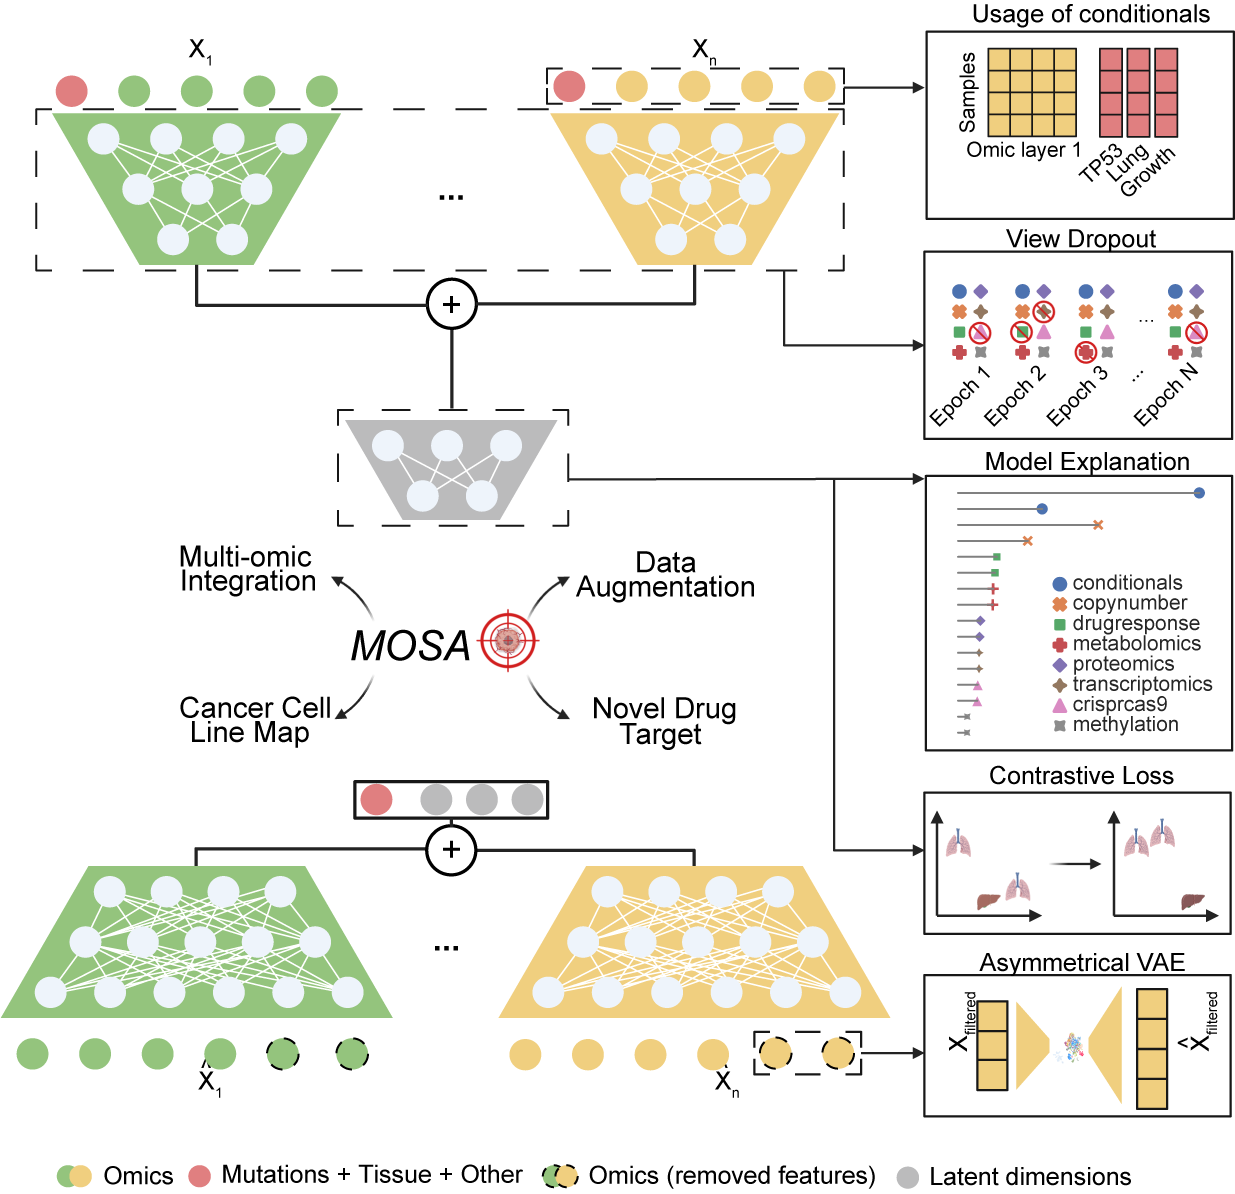
\includegraphics[width=0.5\linewidth]{images/MOSA_Overview.png}
    \caption[MOSA variational autoencoder schematic]{Schematic of the variational autoencoder MOSA, where encoders are represented at the top and decoders at the bottom. Source: \cite{Cai2024}.}
    \label{fig:MOSA_Overview}
\end{figure}

As shown in Figure \ref{fig:MOSA_Overview}, MOSA is implemented as a conditional multi-view variational autoencoder (VAE). Each omic modality, or input view, is first encoded separately using a dedicated encoder. For an input view $i$ with dimensionality $D_i$, the corresponding encoder produces a view-specific latent representation $z_i \in \mathbb{R}^{d_i}$, where $d_i = \lfloor D_i \cdot \texttt{view\_latent\_dim} \rfloor$, with $\texttt{view\_latent\_dim}$ being a configurable model hyperparameter. These modality-specific embeddings are then concatenated to form
\[
z_{\mathrm{concat}} = [z_1; \ldots; z_V] \in \mathbb{R}^{\sum_i d_i},
\]
which is passed through a Gaussian inference block. This block outputs a mean vector $\mu \in \mathbb{R}^{L}$ and a log-variance vector $\log \sigma^2 \in \mathbb{R}^{L}$, from which the joint latent representation is sampled using the reparametrisation trick.

This late-integration strategy allows MOSA to preserve omic-specific information while learning a shared multi-omic representation.

A key feature of MOSA's architecture is its asymmetrical encoder-decoder design, which maintains high predictive capacity while reducing computational complexity. The encoders receive only the most informative features as input. These features are selected using Gaussian mixture models for transcriptomic and methylomic data or significance thresholds for \gls{CRISPR}-Cas9 screens, reducing the number of trainable parameters by 39.2\%. In contrast, the decoders reconstruct the full set of original features for each view, producing per-view reconstructions $\hat{x}_i \in \mathbb{R}^{D_i}$ from the joint latent representation, optionally concatenated with covariates or conditional variables. The model also uses a view-wise dropout, which randomly masks entire omic datasets during training. This prevents over-reliance on any single modality and encourages the model to learn robust relationships across omics.

Additionally, the model includes 237 conditional variables to generate context-specific biological profiles. These variables include cancer driver mutations, tissue types, gene fusions, microsatellite instability status and cell line growth rates. They are incorporated in two stages. First, they are concatenated to each omic layer before encoding, which contextualises the input. They are then concatenated to the joint multi-omic latent representation before decoding to guide condition-specific reconstruction. Missingness is handled using feature-wise masks, allowing reconstructions to be generated for missing values.

The training objective combines configurable per-view reconstruction losses, such as mean squared error or binary cross-entropy, with a KL regularisation term on the joint latent space.

Reconstruction weighting and the overall loss composition are controlled by hyperparameters such as \texttt{w\_rec}, \texttt{w\_kl} or \texttt{beta} and \texttt{view\_loss\_weights}. The implementation further supports explainability through a \texttt{return\_for\_shap} hook that exposes intermediate tensors and the training module provides configurable optimisers and schedulers, early stopping and cross-validation. Through this architecture, MOSA provides a holistic and explainable model for identifying non-linear multi-omic associations and prioritising novel therapeutic targets.